\section{Risultati della stabilizzazione}

\todo{scrivi qualcosa qui, tipo i coefficienti usati}


\subsection{Ottimalità del controllo}
Una volta fissate le matrici nella~\eqref{eq:q-r-matrices},
il regolatore lineare quadratico è ottimale secondo la \autoref{def:lqr}.
Nella \autoref{fig:ottimalità} mostro che scegliendo degli autovalori
stabili arbitrari ottengo sempre un costo finale maggiore.
Nella figura \autoref{fig:non-ottimalità} mostro che,
cambiando funzione costo, LQR smette di essere ottimale.

I valori numerici dei parametri che ho usato
sono riportati in \autoref{tab:parametri-numerici-sistema};
gli autovalori ottimali del sistema $A - BK_{LQR}$ (arrotondati alla terza cifra significativa) sono
\begin{equation}
    \left.
        \begin{aligned}
        &\lambda_1 = -8.56 - 0.019i, \
        &\lambda_2 = -8.56 + 0.018i, \\
        &\lambda_3 = -1.80 - 1.03i, \
        &\lambda_4 = -1.80 + 1.03i.
        \end{aligned}
    \right.
    \label{eq:lqr-eigenvalues}
\end{equation}

\begin{figure}
    \centering
    \begin{subfigure}[t]{.48\textwidth}
        \centering
        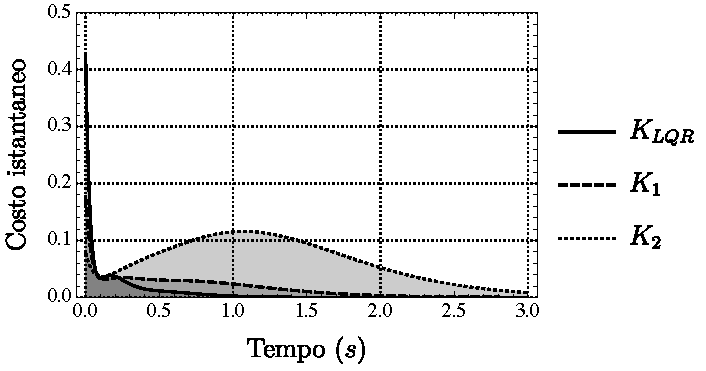
\includegraphics[width=\textwidth]{assets/opt1}
    \end{subfigure}
\hfill
    \begin{subfigure}[t]{.48\textwidth}
        \centering
        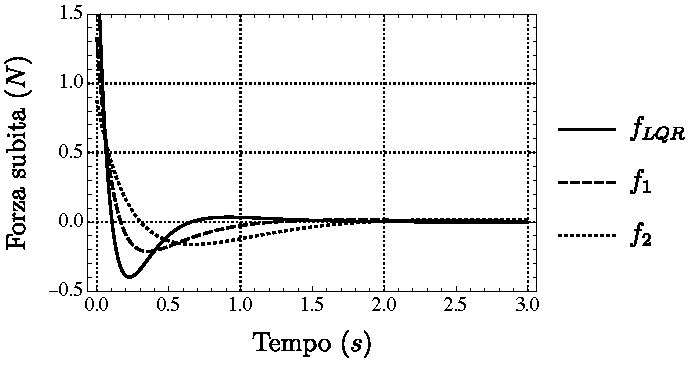
\includegraphics[width=\textwidth]{assets/opt2}
    \end{subfigure}

    \begin{subfigure}[b]{.48\textwidth}
        \centering
        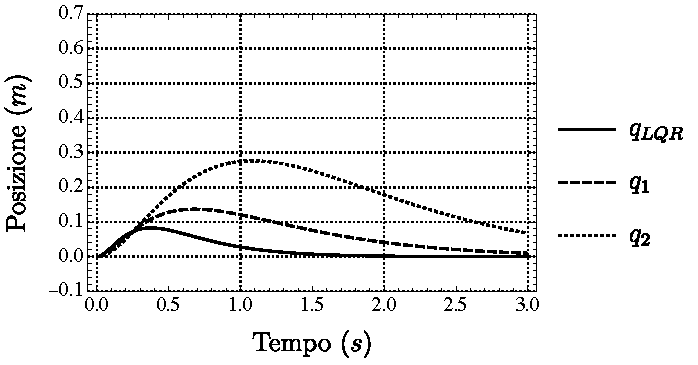
\includegraphics[width=\textwidth]{assets/opt3}
    \end{subfigure}

    \caption[Confronto tra LQR e controlli non ottimali]{
        Confronto tra LQR e strategie di controllo non ottimali.
        $f_1$ è scelta in modo che gli autovalori del sistema
        corrispondano agli~\eqref{eq:lqr-eigenvalues} senza parte
        immaginaria. $f_2$ invece è scelta in modo che il
        sistema abbia autovalori stabili casuali. Entrambe le
        strategie portano ad un costo finale maggiore della strategia
        ottimale $f_{LQR}$. Indicando con $J_i$ il costo di
        una strategia, vale $J_1 \approx 2J_{LQR}$ e $J_2 \approx 8J_{LQR}$.
        In questo caso particolare, $f_{LQR}$ impiega meno tempo di $f_1$ e $f_2$
        a raggiungere $\b 0$.
    }
    \label{fig:ottimalità}
\end{figure}

\begin{figure}
    \centering
    \begin{subfigure}[t]{.48\textwidth}
        \centering
        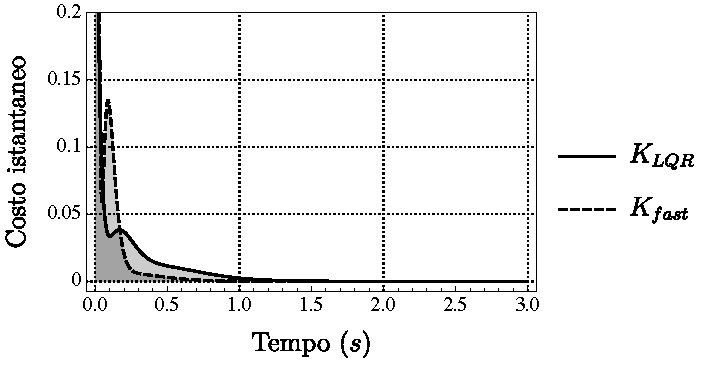
\includegraphics[width=\textwidth]{assets/nopt1}
    \end{subfigure}
    \hfill
    \begin{subfigure}[t]{.48\textwidth}
        \centering
        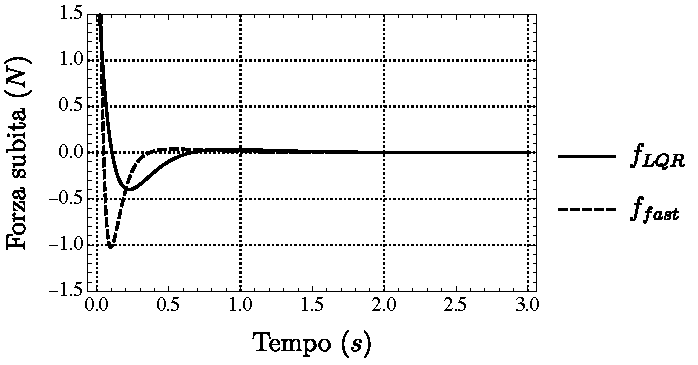
\includegraphics[width=\textwidth]{assets/nopt2}
    \end{subfigure}

    \begin{subfigure}[b]{.48\textwidth}
        \centering
        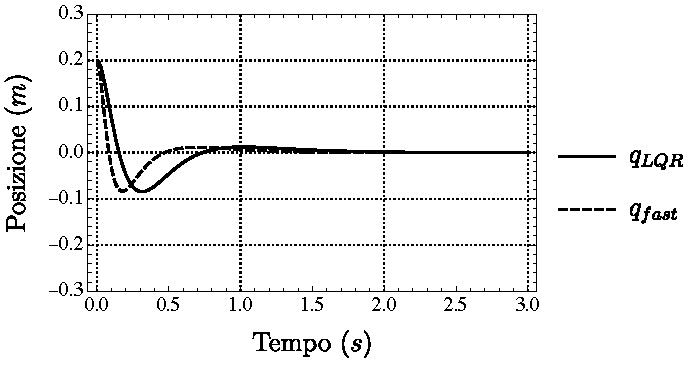
\includegraphics[width=\textwidth]{assets/nopt3}
    \end{subfigure}

    \caption[Confronto tra LQR e un controllo più rapido]{
        Confronto tra LQR e una strategia di controllo differente.
        In questo caso particolare, $f_{fast}$ raggiunge $\b 0$ in minor
        tempo rispetto a $f_{LQR}$, a discapito di un costo più elevato.
    }
    \label{fig:non-ottimalità}
\end{figure}

\subsection{Validità della linearizzazione}
Il sistema non è lineare, quindi mi aspetto che il regolatore lineare quadratico sia
effettivo solamente entro un certo angolo iniziale\footnotemark da $\theta = 0$.
Per ottenere una stima dell'intervallo di validità, espando l'equazione del
moto~\eqref{eq:moto-carrello-theta} in serie di Taylor fino al terzo ordine,
fissando $\dot \theta = 0$.
Sostituendo i valori numerici dei parametri, ottengo
\begin{equation*}
    \frac {\ddot \theta} {\text{cost.}} \approx 4 \theta + \theta^3 + \mathcal O(\theta^4).
\end{equation*}
Mi aspetto che l'approssimazione sia valida quando il termine in $\theta^3$ è
molto minore del termine in $\theta$
\begin{equation}
    \frac{4\theta} {\theta^3} \gg 1.
    \label{eq:rapporto-theta}
\end{equation}

\footnotetext{
    $q$ e $\dot q$ non compaiono nelle equazioni del moto~\eqref{eq:moto-sistema},
    quindi non sono rilevanti per la validità della linearizzazione. Per
    ora considero $\dot \theta(0) = 0$.
}

Ho simulato il sistema usando il regolatore lineare quadratico
con diverse condizioni iniziali e ho trovato che
il sistema smette di essere controllabile quando $|\theta(0)| = \theta_{\max} \approx 1.1$,
quindi quando il rapporto nella~\eqref{eq:rapporto-theta} si avvicina a $3.3$.
I coefficienti di costo $r_{11}$ e $q_{11}$ non influiscono
direttamente sul range di controllabilità, ma possono alterare
il comportamento del sistema quando le condizioni iniziali sono
vicine a $\theta = \theta_{\max}$.
Illustro questo fatto in \autoref{fig:occasional-blowup}.

Attraverso le simulazioni ho osservato che l'unica variabile
significativa per la controllabilità è $\theta$.
Posso stimare ugualmente un valore massimo per le altre
variabili considerando l'energia che il sistema ha nello stato
\begin{equation*}
    \b x = (0, 0, \theta_{\max}, 0)
\end{equation*}
e stimando che, perchè il sistema sia controllabile,
l'energia debba essere minore di questo valore.

Il sistema reale si comporta in modo simile.
In \autoref{fig:real-theta-limit} sono mostrati alcuni set di dati
con condizioni iniziali date da valori crescenti di $\theta(0)$.
Partendo da fermo, il sistema riesce a raggiungere l'equilibrio quando
$\theta(0) < 1$.

\begin{figure}
    \vskip 0pt
    \centering
    \begin{subfigure}[t]{0.48\textwidth}
        \centering
        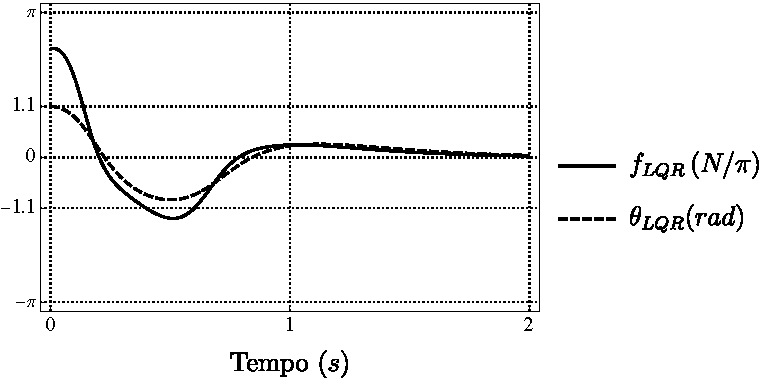
\includegraphics[width=\textwidth]{assets/occasional-blowup-r1}
        \caption{$r_{11} = 1$. Il sistema riesce a tornare a $\b x = \b 0$.}
        \label{fig:does-not-blowup}
    \end{subfigure}
    \hfill
    \begin{subfigure}[t]{0.48\textwidth}
        \centering
        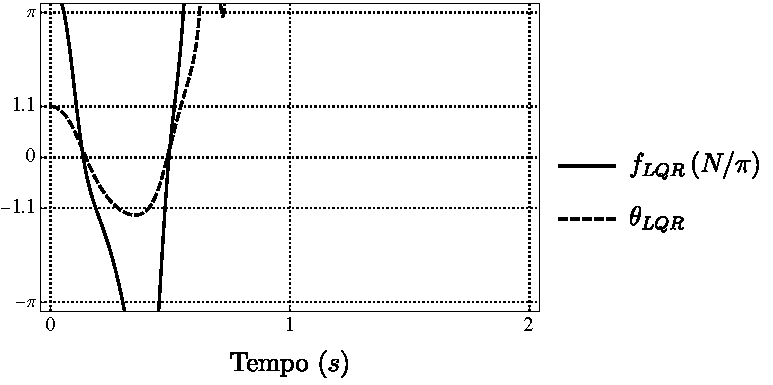
\includegraphics[width=\textwidth]{assets/occasional-blowup-r.1}
        \caption{$r_{11} = .1$. Il sistema risponde troppo
            aggressivamente, $\theta$ supera $\theta_{\max}$ e la soluzione diverge.}
        \label{fig:does-blowup}
    \end{subfigure}
    \caption[Dipendenza delle soluzioni dalla funzione costo]{
        Dipendenza delle soluzioni dai coefficienti della funzione costo
        per condizioni iniziali vicine a $\theta = 0$.
        Le due simulazioni nelle Figure~\ref{fig:does-not-blowup} e~\ref{fig:does-blowup}
        hanno entrambe come condizione iniziale $\b x = (0, 0, 1, 0)$ ma
        hanno diversi coefficienti $r_{11}$ per la funzione costo.
    }
    \label{fig:occasional-blowup}
\end{figure}


\begin{figure}
    \vskip 0pt
    \centering
    \begin{subfigure}[t]{0.48\textwidth}
        \centering
        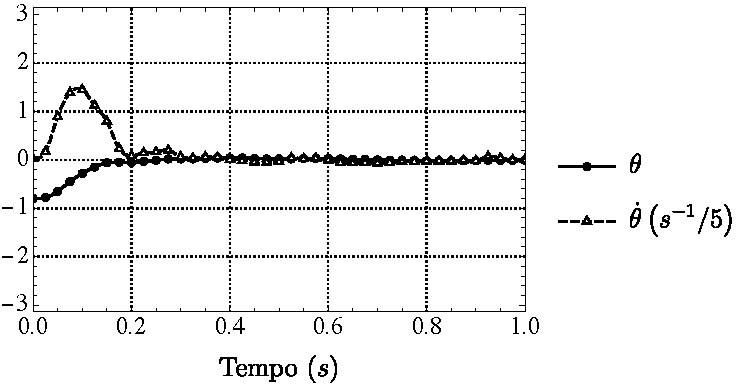
\includegraphics[width=\textwidth]{assets/theta-limit-angle8}
        \caption{$\b x_0 = (0, 0, .8, 0)^\T$}
    \end{subfigure}
    \hfill
    \begin{subfigure}[t]{0.48\textwidth}
        \centering
        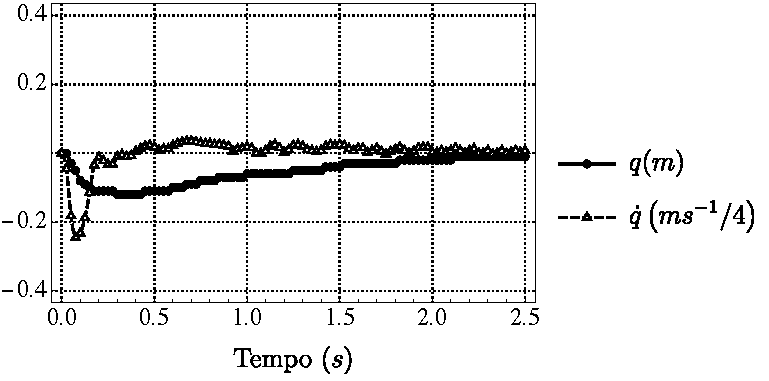
\includegraphics[width=\textwidth]{assets/theta-limit-pos8}
        \caption{$\b x_0 = (0, 0, .8, 0)^\T$}
    \end{subfigure}

    \centering
    \begin{subfigure}[t]{0.48\textwidth}
        \centering
        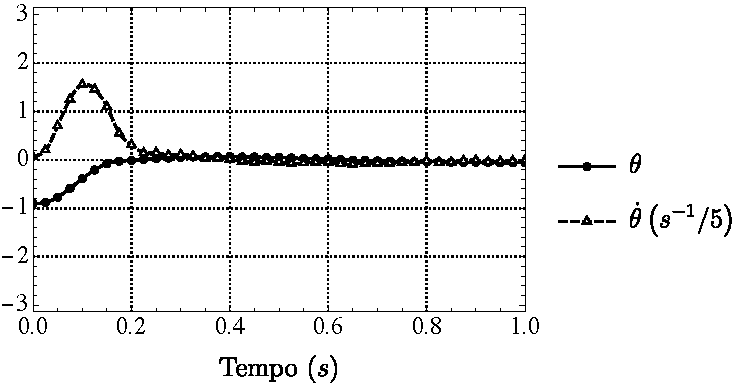
\includegraphics[width=\textwidth]{assets/theta-limit-angle9}
        \caption{$\b x_0~=~(0, 0, .9, 0)^\T$}
    \end{subfigure}
    \hfill
    \begin{subfigure}[t]{0.48\textwidth}
        \centering
        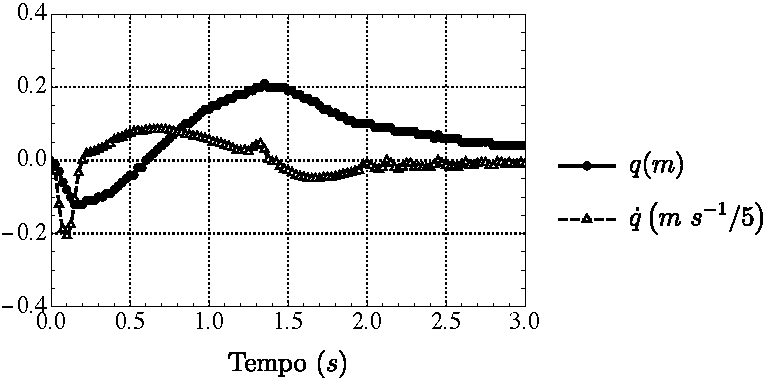
\includegraphics[width=\textwidth]{assets/theta-limit-pos9}
        \caption{$\b x_0 = (0, 0, .9, 0)^\T$}
\end{subfigure}

    \centering
    \begin{subfigure}[t]{0.48\textwidth}
        \centering
        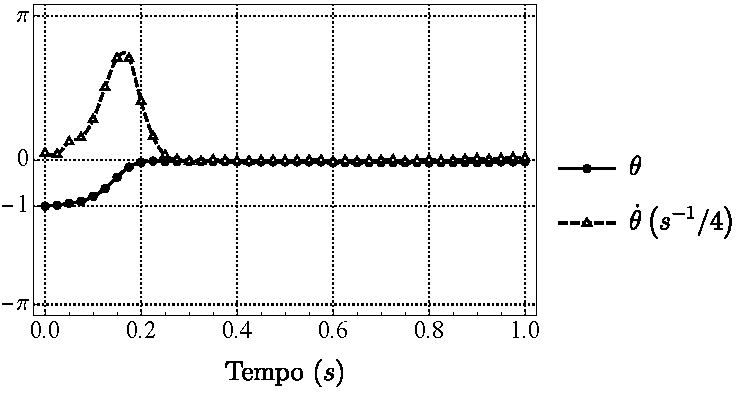
\includegraphics[width=\textwidth]{assets/theta-limit-angle1}
        \caption{$\b x_0 = (0, 0, 1, 0)^\T$}
    \end{subfigure}
    \hfill
    \begin{subfigure}[t]{0.48\textwidth}
        \centering
        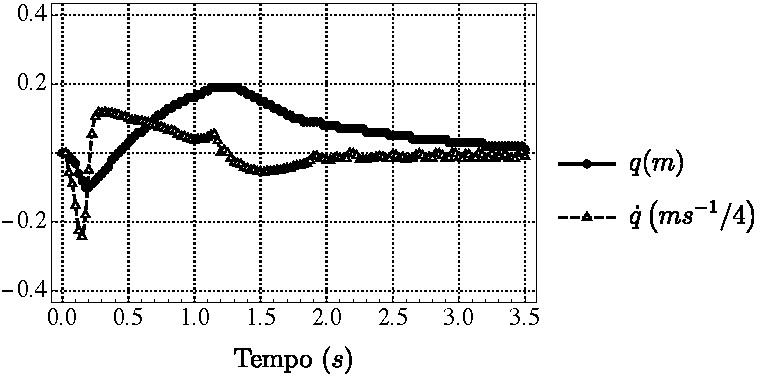
\includegraphics[width=\textwidth]{assets/theta-limit-pos1}
        \caption{$\b x_0 = (0, 0, 1, 0)^\T$}
    \end{subfigure}


    \caption[Limite della validità della linearizzazione]{
        Prove per verificare il limite angolare
        della validità del modello.
        I grafici a sinistra mostrano i dati di angolo e velocità angolare,
        quelli a destra i dati di posizione e velocità e sotto i singoli grafici sono
        riportate le condizioni iniziali, con $\b x_0 = \b x(0)$.
        I grafici sono costruiti in modo da rappresentare l'intervallo
        possibile di valori per $\theta$ e $q$; le velocità sono
        state riscalate per rientrare nei grafici.
        In tutti i set di dati l'angolo viene immediatamente riportato
        a zero, mentre il sistema impiega un tempo sempre crescente
        per azzerare posizione e velocità.
    }
    \label{fig:real-theta-limit}
\end{figure}


\subsection{Confronto tra modello e sistema reale}